\section{System Architecture}

\subsection{Implementation Overview}

While implementing the Kademlia DHT, our focus was to create a modular and extensible system, that can easily be maintained and expanded upon in the future.
To achieve this, we sought to seperate out as many components as possible, keeping each file and package focused on a single responsibility, while also utilizing 
handlers to abstract away the underlying implementation details of each component. This approach allows us to easily swap out components, such as the network layer, 
without affecting the rest of the system.

\subsection{Implementation Details}
One important aspect of our implementation is how we handle docker swarm mode to spin up multiple instances of our Kademlia node and form a network. Each node needs to know the IP address and the ID of a node to join the network via that node. To facilitate this, we chose to use a bootstrap node, which is a already known node in the network that all subsequent nodes can connect to. This bootstrap node is started first, and has a hard coded ID in the docker compose file, but can easily be exchanged for any other ID by changing the docker compose fil to use a environment variable instead. All other nodes are then started and knows the docker service name of the bootstrap node and gets its ID via a CLI flag when started. This way, all nodes can connect to the bootstrap node and join the network.



\subsection{System Architecture Diagram}
A high level system architecture diagram is shown in Figure \ref{fig:architecture}. The diagram illustrates the main components of the Kademlia system and some of their interactions. Note, this is a simplified view of the system and does not include all components and interactions. The main components are described below:
\begin{itemize}
    \item \textbf{Network Layer:} This layer handles all network communications, including sending and receiving messages between nodes. It abstracts away the underlying network implementation, allowing for easy replacement or modification. As of now, there exists a mock network implementation for testing purposes as well as a UDP based implementation for actual network communication.
    \item \textbf{Kademlia Node:} This component represents a single node in the Kademlia network. It manages its routing table, handles incoming requests, and initiates outgoing requests to other nodes.
    \item \textbf{Routing Table:} The routing table is responsible for maintaining a list of known nodes in the network. It organizes nodes into buckets based on their distance from the current node, facilitating efficient lookups and routing. This implementation does not implement the correct binary tree structure as described in the Kademlia paper, but rather uses a simpler list based approach for storing nodes in each bucket (given by the lab instructions).
    \item \textbf{Message Handlers:} These components are responsible for processing incoming messages and executing the appropriate actions based on the message type (e.g., PING, STORE, FIND VALUE). There also exsists temporary message handlers which are used for waiting for responses to outgoing requests, such as waiting for a PONG response after sending a PING request. These temporary handlers are removed once the response is received or a timeout occurs. But they are removed from the diagram for simplicity.
    \item \textbf{Command Line Interface (CLI):} The CLI provides an interactive interface for users to interact with the Kademlia node, allowing them to execute commands such as joining the network, storing values, and retrieving values.

\begin{figure}[htbp]
    \centering
    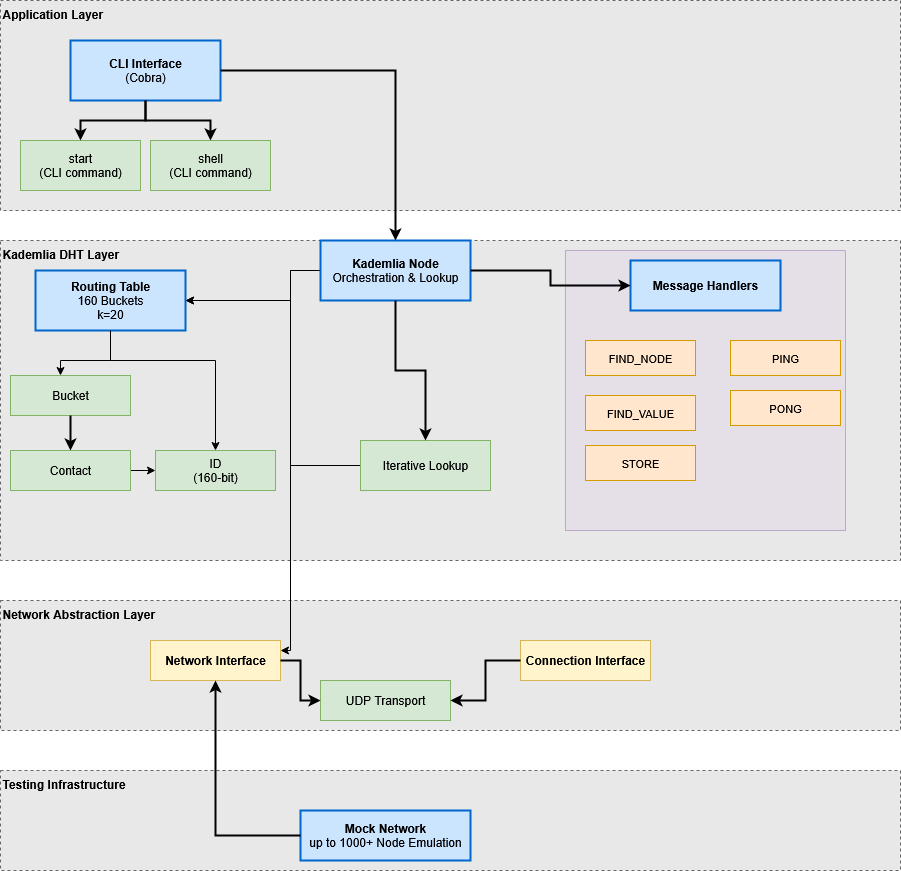
\includegraphics[width=0.8\textwidth]{Images/component_diagram.drawio.png}
    \caption{Component diagram of the Kademlia DHT system showing the layered architecture and component relationships.}
    \label{fig:architecture}
\end{figure}

